\chapter{性能验证和实验结果}

我们提出的粗粒度稀疏的神经网络加速器能够充分利用粗粒度稀疏神经网络的神经元/索引共享和负载均衡等特性,同时利用动态神经元稀疏和局部量化进一步减少计算量和访存量,从而提升加速器性能,减少能耗。

我们采用模拟的方法对新型加速器进行性能分析。传统的周期精确模拟器由于性能低,速度满,无法满足我们实际的需求,因此,我们为新型加速器设计了一个专用性能模拟器,它能够在误差允许范围内快速进行性能模拟。该性能模拟器基于事件驱动进行设计,它能够隐藏加速器中复杂的设计细节,专注于影响加速器性能的因素,从而快速,准确地预测神经网络在新型加速器上的执行时间。

最后我们在七个benchmark上分别比较了CPU,GPU,DianNao,Cambricon-X和新型加速器的性能和能耗,我们发现新型加速器具有高性能和低能耗的特点。与最先进的稀疏的神经网络加速器Cambricon-X相比,新型加速器能够获得1.71倍的加速比,同时减少1.75倍的能耗。在65nm工艺下,新型加速器面积和功耗仅仅为$6.82mm^2$和$821.19mW$。

\section{新型加速器性能验证}

\subsection{背景}
计算机模拟是指利用计算机软件开发的模拟器对真实世界过程或者系统进行模拟的行为,进而完成故障分析、测试 VLSI逻辑设计等复杂的任务,从而为研究人员提供设计指导。计算机系统模拟器是指以在一台计算机上模拟另一台指令不兼容或者体系不同的计算机。如今,计算机系统模拟器已经成为了计算机系统结构领域研究中不可或缺的工具。研究人员通过使用模拟器能够用较低的成本和开销,高效地完成对软硬件的配置和观察,进而为硬软件的设计和优化提供指导。随着计算机行业的迅猛发展,计算机功能变得越来越强大的同时,计算机系统也变得越来越复杂,模拟计算机系统的开销也越来越大,因此如何提升模拟器的性能成为一个亟待解决的问题。研究者一般从准确性,事件开销,内存开销,易用性和可扩展性这几个方面考虑模拟器的性能。

研究者一般采用周期精确模拟器进行硬件的性能模拟。周期精确模拟器需要模拟硬件的每一个模块在每一个时钟周期执行操作的各个细节,包括状态机跳转,寄存器更改,流水级操作等,以保持模拟器与硬件之间的一致性。这种精确模拟会导致巨大的资源,能源和时间开销,进而导致周期精确的模拟器无法满足实际的需求。

周期精确的模拟器按照实现方式可以分为两类,一类是时间触发的模拟器,一类是事件触发的模拟器。其中时间触发模拟器以cycle为单位进行模拟,每一个cycle会触发一次模拟操作;事件触发模拟器以事件为单位进行模拟,事件通常为用户自定义事件,每一个事件会触发一次模拟操作。如图~\ref{}所示,一个浮点乘法单元需要产生一个浮点乘法操作,该浮点乘法需要四个周期完成。当我们使用时间触发的模拟器时,总共需要五个周期模拟浮点乘法操作,尽管第二,三,四周期内不需要进行任何模拟操作;当我们使用事件触发的模拟器时,只需要两个周期就能够完成。由于神经网络加速器涉及到大规模数据的传输和运算,基于事件触发的模拟器更有性能上的优势。

\subsection{加速器专用性能模拟器}

我们采用基于事件触发的模拟器对新型加速器进行性能模拟。在设计性能模拟器的过程中,我们采用了如下的策略优化模拟器,在误差允许范围内加快模拟速度,提高模拟器的性能:第一,我们对加速器进行高层次抽象,隐藏加速器中复杂的细节,只关注影响性能的最主要因素,从而简化性能模拟器的设计,加快性能模拟器的模拟速度。第二,我们精简了模拟器中的事件,提取出最重要的事件构建神经网络的执行过程,同时我们使用建模的方法计算事件的执行时间,提高模拟器的准确性。第三,我们根据loop tiling将神经网络的执行过程分为多个子运算,然后我们以子运算为单位进行性能模拟,最终通过累加各个子运算的执行事件获得神经网络在加速器上的运行时间。


\subsubsection{加速器的高层次抽象}

\begin{figure}[h]
\centering
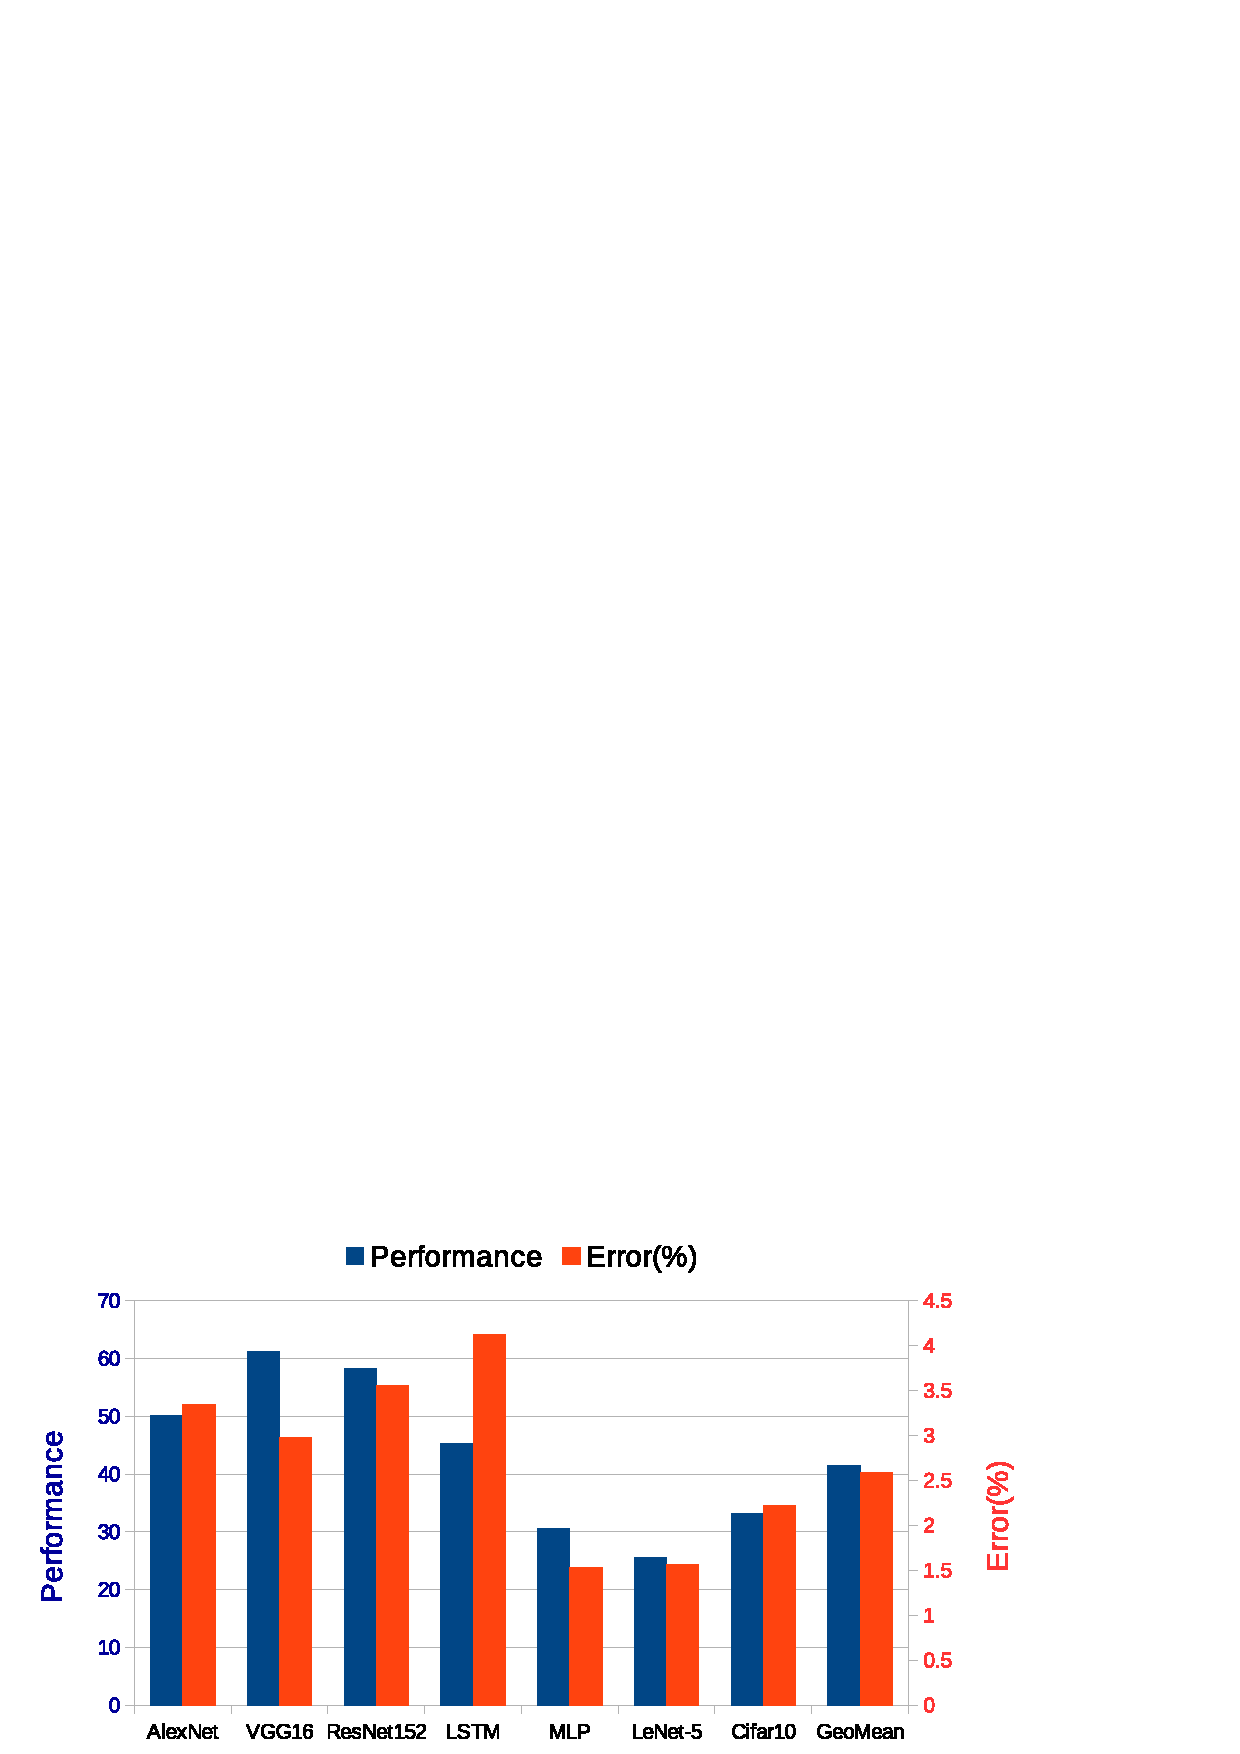
\includegraphics[width=1.0\columnwidth]{simulator.pdf}
\caption{加速器的抽象结构}
\label{fig:simulator}
\end{figure}

为了简化性能模拟器的设计,加快性能模拟器的模拟速度,我们首先需要对新型加速器进行高层次的抽象,隐藏新型加速器的细节,提取出影响神经网络执行速度的关键因素。由于新型加速器中的大部分模块内部采取流水(pipeline)的方式执行,而且部分模块之间也完成了流水操作,因此我们可以将这些流水的模块整合为一个大模块,从而隐藏新型加速器的设计细节。

如图~\ref{fig:simulator}所示,新型加速器的抽象结构由三部分构成,分别是Main Block, Sub Block和Off-chip Memory。Main Block内部由片上缓存SRAM,运算单元FU(functional unit)组成,Sub Block由片上缓存运算SSRAM和运算单元FU构成。

Off-chip Memoy存储了神经网络的参数,包括神经网络的拓扑结构,输入,权值,部分和,输出等。由于加速器的片上缓存有限,加速器无法一次性将神经网络的所有参数存储到片上缓存,因此Off-chip Memory与片上缓存之间需要由非常频繁的数据交换。

Main Block主要作为数据通路同时,完成一部分向量运算和标量运算。它的内部集成了新型加速器中的选数逻辑,由于选数逻辑与运算逻辑之间为流水的结构,因此我们将这部分选数逻辑隐藏。
Main Block中的SRAM对应了新型加速器中的四个片上缓存,分别是NBin,NIBin,NBout和SIB。Main Block中的FU主要用来完成向量运算和标量运算,其中向量运算包括逐元素相加,逐元素相乘等运算,标量运算包括标量四则运算。Main Block中主要完成Pooling层,BN层和ROI Pooling层的运算。

Sub Block主要是核心运算模块,主要完成神经网络算法中的矩阵向量运算。Sub Block中的SRAM对应新型加速器中的SB,FU则对应了PEFU。神经网络中的卷积层,全连接层和LSTM层的大部分运算都在Sub Block的FU中完成。

Main Block与Sub Block之间存在数据双向的数据通路,从Main Block到Sub Block方向的通路用来传输输入神经元,从Sub Block到Main Block方向的通路用于传输输出神经元部分和。
Main Block与Off-chip Memory之间也存在双向数据通路,其中从Off-chip Memory到Main Block方向的通路用来加载输入神经元,输入神经元索引,输出神经元部分和和权值索引,从Main Block到Off-chip Memory方向的通路用来存储输出神经元部分和。
Sub Block与Off-chip Memory之间仅仅存在单向的数据通路,从Off-chip Memory到Sub Bloock方向的通路用来加载权值。

值得注意的是,抽象的加速器结构隐藏了选数模块,WDM模块和Encoder模块,主要是因为这些模块与计算模块之间是组成了流水级,只要我们能够准确模拟运算模块的性能,是否模拟这些模块对最终的结果没有影响,因此我们可以隐藏这些模块的细节,专注于加速器中运算模块的模拟。

\subsubsection{事件分类}

设计基于事件触发的模拟器,我们首先需要根据加速器的特性和数据流定义在加速器在运行神经网络过程涉及到的事件。事件有一个四维的描述符,分别是类型,数据,时刻和事件,其中类型用来描述事件需要完成的操作,包括控制(如分支跳转),访存(如Load/Store片外DDR或者Read/Write片上缓存),运算(如矩阵,向量,标量,逻辑运算等);数据描述事件涉及到的数据,包括数据地址,数据大小,数据类型等信息;时刻描述了事件出触发的时间点;事件描述了事件的执行时间,执行时间可以通过性能分析(Profiling)或者建模(Modeling)的方式完成。

我们在新型加速器的性能模拟器中定义了四个事件,分别是数据加载事件,运算事件,数据存储事件和同步事件,我们将它们依次简写为Load事件,Compute事件,Store事件和Synchronize事件。

Load事件涉及到将数据从Off-chip Memory加载到Main Block的SRAM和Sub Block的SRAM中;对应到新型加速器中,就是将输入神经元,输入神经元索引,输出部分和,权值和权值索引分别从片外加载到NBin,NIBin,NBout,SB和SIB中。

Compute事件涉及到Main Block中的FU和Sub Block中的FU完成神经网络的核心运算,神经网络运算包括矩阵运算,向量运算和标量运算,其中矩阵运算主要包括矩阵向量运算,这部分是神经网络的核心运算,卷积层,全连接层,LSTM层中大部分运算都是矩阵向量运算;向量运算包括向量内积,向量逐元素相乘,向量逐元素相乘,神经网络中的池化层,BN层,LSTM层,LRN层等都是涉及到向量运算;标量运算主要包括标量的四则运算,Faster-RCNN中的ROI pooling层会涉及到这部分的运算。因此,Compute事件还能进一步划分矩阵运算事件(Matrix Compute),向量运算事件(Vector Compute)和标量运算事件(Scalar Compute)。

Store事件涉及到将Main Block SRAM中的数据存储到Off-chip Memory;对应到新型加速器中,就是将输出部分和从NBout存储回Off-chip Memory。值得注意的是NBin,NIBin,SB和SIB这四个缓存不会涉及到Store事件。

Synchronize事件是一个同步事件,当出现Synchronize事件时,必须要保证Synchronize事件之前其他所有事件完成才能执行Synchronize事件之后的其他事件,也就是说Synchronize事件相当与一个同步信号,用来同步Synchronize事件之前的其他事件。

\subsubsection{事件执行时间}
下面我们将介绍如何模拟各个事件执行的时间。

Load事件的执行时间跟数据量和Off-Chip Memory带宽有关,具体可以用如下方式进行计算
\begin{equation}
t_{Load} = t_{start} + Data_{Load} / Bandwidth_{Load}
\end{equation}
其中$t_{Load}$是Load事件执行时间,$t_{start}$是Off-chip Memory的启动时间,$Data_{Load}$是Load事件涉及到的数据量(包括所有输入神经元,输入神经元索引,输出部分和,权值和权值索引),$Bandwidth_{Load}$是Off-Chip Memory的Load带宽。

Compute事件的执行时间与运算量和运算单元数量有关,具体可以用如下方式进行计算
\begin{equation}
t_{Compute} = Data_{Compute} / (FU * u\%)
\end{equation}
其中$t_{Compute}$是Compute事件执行时间,$Data_{Compute}$是Compute事件涉及的运算量,$FU$是运算单元的数量,$u\%$是运算单元的利用率。神经网络神经元稀疏度,权值稀疏度,网络拓扑结构(如卷积层的规模,全连接层的规模)数据阻塞等因素都会影响运算单元的利用率,因此运算单元的利用率是一个实时的值。我们采用建模的方法计算运算单元的利用率进行预测,例如对于神经网络的卷积运算,我们会实测多组不同网络规模配置和稀疏度配置下运算单元利用率,然后根据这些数据对运算单元利用率进行建模,最终获得运算单元利用率与网络配置和稀疏度的定量关系。值得注意的是Matrix Copmute事件,Vector Compute事件和Scalar事件的执行时间都可以用上述公式进行计算。

Store事件的执行时间计算方法与Load时间类似,执行时间跟数据量和Off-Chip Memory带宽有关,具体可以用如下方式进行计算
\begin{equation}
t_{Store} = t_{start} + Data_{Store} / Bandwidth_{Store}
\end{equation}
其中$t_{Store}$是Store事件执行事件,$t_{start}$是Off-chip Memory的启动时间,$Data_{Store}$是事件涉及到的数据量(输出部分和),$Bandwidth_{Store}$是Off-Chip Memory的Store带宽。

Synchronize事件是一个阻塞事件,用于同步之前所有的事件,因此不需要计算其执行时间。


\subsubsection{事件的依赖关系}
由于新型加速器中集成了多发射控制器~\ref{subsec:control},因此新型加速器可以同时发射没有依赖关系的指令。在新型加速其中,没有依赖关系的指令包括三个方面,第一,IO指令与计算指令之间没有依赖关系;第二,Load和Store指令之间没有依赖关系;第三,如果计算指令涉及到涉及不同的计算单元和数据,那么这些计算指令之间也没有依赖关系。

对应的,性能模拟器也存在没有依赖关系的事件:第一,Load/Store事件与Compute事件之间没有依赖关系;第二,Load事件与Store事件之间没有依赖关系;第三,Matrix Compute事件,Vector Compute事件和Scalar事件之间没有依赖关系。没有依赖关系的事件可以同时执行,我们用Synchronize事件来同步没有依赖关系的事件。

\subsubsection{模拟过程}

\begin{figure}[h]
\centering
\includegraphics[width=1.0\columnwidth]{simulation.pdf}
\caption{性能模拟器模拟神经网络在加速器上的执行过程}
\label{fig:simulation}
\end{figure}

我们使用loop tiling的策略将神经网络运算分割成为多个子运算操作,使得每一个子运算对应的数据能够被完整加载到片上缓存中。假设神经网络某一层的运算被切分成为\emph{N}个子运算,同时\emph{N}个子运算对应\emph{N}个数据块。如图~\ref{fig:simulation}描绘了模拟器模拟神经网络在加速器上执行,同时统计运行时间的过程。神经网络的执行过程被分为\emph{N+2}个\emph{Step},两个\emph{Step}之间用\emph{Synchronize}事件进行分割,最终神经网络的执行时间是这\emph{N+2}个\emph{Step}的执行事件总和。

\emph{Step 1}:性能模拟器会触发\emph{Load 1}事件。\emph{Load 1}事件将第一个子运算对应的数据从Off-chip Memory加载到Main Block和Sub Block的SRAM中。此时由于片上缓存没有数据,Main Block和Sub Block的FU无法进行计算。然后我们使用\emph{Synchronize}事件进行同步。\emph{Step 1}的执行时间就是\emph{Load 1}事件执行时间。

\emph{Step 2}: 性能模拟器触发\emph{Load 2}事件和\emph{Compute 1}事件。其中\emph{Load 2}事件将第二个子运算对应的数据从Off-chip Memory加载到Main Block和Sub Block的SRAM中。此时由于片上缓存已经存储了第一个子运算对应的数据(经过\emph{Step 1}的\emph{Load 1}事件),所以模拟器会触发\emph{Compute 1}事件,Main Block和Sub Block的FU完成第一个子运算。值得注意的是,\emph{Compute 1}事件包括\emph{Matrix Compute 1}事件,\emph{Vector Compute 1}事件和\emph{Scalar Compute 1}事件这三个没有依赖关系的事件。最终\emph{Step 2}的执行时间取决于\emph{Load 1}, \emph{Matrix Compute 1}, \emph{Vector Compute 1}和\emph{Scalar Compute 1}这四个事件的执行时间的最大值。
为了表示方便,我们将\emph{Computen i}事件执行时间定义为\emph{Matrix Compute i}, \emph{Vector Compute i}和\emph{Scalar Compute i}这三个事件中执行时间的最大值。

\emph{Step 3}: 性能模拟器触发\emph{Load 3}事件,\emph{Compute 2}事件和\emph{Store 1}事件。其中\emph{Load 2}事件将第二个子运算对应的数据从Off-chip Memory加载到Main Block和Sub Block的SRAM中。\emph{Compute 2}事件开启Main Block和Sub Block的FU完成第二个子运算。 此时,由于Main Block的SRAM中存储了第一个子运算对应的结果(经过\emph{Step 2}的\emph{Compute 1}事件),模拟器触发\emph{Store 1}事件,将第一个子运算的运算结果存储到Off-Chip Memory。
最终\emph{Step 3}的执行时间是\emph{Load 3}, \emph{Compute 2}和\emph{Store 1}这三个事件执行时间的最大值。

......

\emph{Step i+1}:性能模拟器触发\emph{Load i+1}事件,\emph{Compute i}事件和\emph{Store i-1}事件,它们分别将第\emph{i+1}个子运算对应的数据从Off-chip Memory加载到片上缓存,计算第\emph{i}个子运算,将第\emph{i-1}个数据块从片上缓存存储到Off-chip Memory中。\emph{Step i+1}的执行时间是\emph{Load i+1}, \emph{Compute i}和\emph{Store i-1}这三个事件执行时间的最大值。

......

\emph{Step N}:性能模拟器触发\emph{Load N}事件,\emph{Compute N-1}事件和\emph{Store N-2}事件。它们分别将第\emph{N}个子运算对应的数据从Off-chip Memory加载到片上缓存,计算第\emph{N-1}个子运算,将第\emph{N-2}个数据块从片上缓存存储到Off-chip Memory中。从\emph{Step 1}到\emph{Step N},性能模拟器将神经网络的N个子运算涉及的数据加载到片上缓存。

\emph{Step N+1}:性能模拟器触发\emph{Compute N}事件和\emph{Store N-1}事件。它们分别计算第\emph{N}个子运算,将第\emph{N-1}个数据块从片上缓存存储到Off-chip Memory。从\emph{Step 2}到\emph{Step N+1},性能模拟器完成了神经网络的N个子运算的计算任务。

\emph{Step N+2}: 性能模拟器出发\emph{Store N}事件将第N个子运算的计算结果从片上缓存存储到Off-chip Memory。从\emph{Step 3}到\emph{N+2},性能模拟器将神经网络N个子运算的计算结果存储到Off-chip Memory。至此,性能模拟器完成了神经网络的所有运算。

\section{实验方法}
在本节中,我们介绍新型稀疏神经网络加速器相关的实验方法。

我们使用Synopsys工具链中的TMSC 65nm库对加速器的RTL实现进行综合。我们使用CACTI 6.0预测DRAM访存能耗~\cite{muralimanohar2007optimizing}。我们使用基于PrimeTime PX的VCD波形文件评估能耗。最后我们使用基于事件触发的模拟器评估加速器的性能。

\subsection{Baseline}
我们将加速器与CPU,GPU和硬件加速器进行比较。

\subsubsection{CPU}
我们使用目前流行的深度学习框架Caffe~\cite{jia2014caffe}评估神经网络在CPU上的性能。CPU的型号是拥有6核的英特尔志强 E5-2620 v2,工作频率为$2.1GHz$,工艺为$22nm$。同时,我们使用稀疏库(sparse-BLAS)~\cite{duff2002overview}来评估稀疏神经网络的性能。我们用CPU-Caffe和CPU-Sparse分别表示稠密网络和稀疏网络在CPU上的性能。

\subsubsection{GPU}
我们使用Caffe评估神经网络在GPU上的性能(用GPU-Caffe表示)。GPU的型号是Nvidia K20,拥有5GB GDDR5,峰值能够达到$3.52TFlops$,工艺为$28nm$。同时我们使用cuBLAS来实现神经网络算法(用GPU-cuBLAS表示)。最后,我们使用先进的cuSparse库评估稀疏神经网络的性能(用GPU-Sparse表示)。

\subsubsection{硬件加速器}
我们将新型加速器与目前最先进的神经网络加速器DianNao和Cambricon-X进行性能比较。DianNao拥有很小的步长和很高的吞吐量,能够加速大多数的CNN和DNN。Cambricon-X是一个稀疏神经网络加速器,它能够利用稀疏特性提高性能同时降低能耗。我们选择Cambricon-X作为baseline,主要是考虑到它能够最大程度利用稀疏特性,并且具有通用性。考虑到稀疏利用率,对比稠密神经网络,Cambricon-X通过挖掘稀疏性能够获得2.93倍的加速比,而Cnvlutin和SCNN分别只能获得1.37倍和2.7倍的加速比。考虑到通用性,SCNN在全连接层上的性能非常低,而EIE只能用来加速稀疏的全连接层。

\subsection{Benchmark}
如表~\ref{tab:compression}所示,我们使用七个代表神经网络:AlexNet, VGG16, LeNet-5,MLP,Cifar10,ResNet-152和LSTM作为benchmark。值得注意的是,我们表中参数都是经过粗粒度剪枝后的网络参数。

\section{实验结果}

\subsection{硬件属性}

在当前的加速器中,为了兼容剪枝块的大小,我们将PE的数量$T_n$以及每个PE内部乘法器数量$T_m$配置为$T_n = T_m = 16$,同时考虑到神经网络神经元和权值的稀疏度,我们将NSM设计为256选16的结构,SSM设计为64选16的结构,Encoder设计为64选16的结构。新型加速器的布局特点,各模块的面积和功耗如表~\ref{tab:hardware}所示。加速器的总面积和总功耗分别是$6.82mm^2$和$821.19mW$,工作频率为1GHz,吞吐量为512GOP/s,片上SRAM共为$54KB$。新型加速器的面积分别是Cambricon-X($6.38mm^2$)和DianNao($3.02mm^2$)的1.07倍和2.26倍,同时功耗比Cambricon-X($954mW$)低$132.81mW$,比DianNao($485mW$)高$336.19mW$。
值得注意的是,我们当前加速器并不包含熵解码模块,因此不支持经过熵编码后的神经网络~\ref{subsubsec:encoidng_hw }。

\begin{table}[h]
\caption{加速器详细属性}
\centering
\label{tab:hardware}
\begin{tabular}{lllllllllllll}
\toprule
 & Area($mm^2$) & \% & Power(mW) & \% \\
\midrule
Total   & 6.82	& 100.00\% 	& 821.19    & 100.00\% \\
\midrule
NBin    & 0.55  & 8.06		& 93.32     & 11.36	\\
NBout   & 0.55  & 8.06	    & 93.32     & 11.36	\\
SIB     & 0.05 	& 0.73		& 6.89      & 0.84	\\
NIB     & 0.05  & 0.73      & 6.89      & 0.84  \\
CP      & 0.16 	& 2.35		& 75.06     & 9.14	\\
NSM     & 0.69 	& 10.12		& 121.46    & 14.79	\\
Encoder & 0.04  & 0.60      & 15.75     & 1.92  \\
NFU     & 4.73 	& 69.35 	& 408.50    & 49.75	\\
~~~SB   & ~~~1.05 	& ~~~22.20	& ~~~151.91 & ~~~37.19\\
~~~SSM  & ~~~0.25 	& ~~~5.29	& ~~~56.80  & ~~~13.90	\\
~~~WDM  & ~~~1.54 	& ~~~32.56	& ~~~16.25  & ~~~3.98	\\
~~~PEFU & ~~1.89	& ~~~33.95	& ~~~183.54 & ~~~44.93 \\
\bottomrule
\end{tabular}
\end{table}

此外,新型加速器处理稀疏和量化模块(NSM, SSMs, Encoder和WDM)的面积和功耗分别是$2.52mm^2$(占总面积的$36.95\%$)和$210.26mW$(占总功耗的$25.60\%$),却能够获得比Cambricon-X高的1.71倍性能,同时降低1.75倍的能耗。值得注意的是,即使新增了突触选择模块,新型加速器的索引模块(即NSM和SSM)的面积对比与Cambricon-X的IM模块减少了2.11倍($0.94mm^2$ vs. $1.98mm^2$),功耗减少了1.87 倍($178.26mW$ vs. $332.62mW$);同时新型加速器的NSM的面积和功耗分别是Cambricon-X中IM模块的$36.52\%$和$34.85\%$,却实现了与IM模块相同的功能(即筛选神经元)。因此,我们的设计对比于Cambricon-X在面积,能耗上都有很大的提升。

\subsection{性能}
在表~\ref{tab:compression}所列出的七个benchmark上,我们比较了新型加速器,CPU,GPU,DianNao和Cambricon-X的性能。在CPU和GPU上,我们同时评估稀疏神经网络和稠密神经网络的性能,即我们使用稀疏库(CPU-Sparse,GPU-Sparse)评估稀疏神经网络的性能,使用稠密库(CPU-Caffe, GPU-Caffe, GPU-cuBLAS)评估稠密神经网络的性能。为了与CPU和GPU公平比较,我们评估了加速器在稠密网络上的性能(ACC-dense)。同时为了与Cambricon-X和DianNao公平比较,我们评估了这三个加速器在稀疏神经网络上的性能。

\begin{figure}[h]
\centering
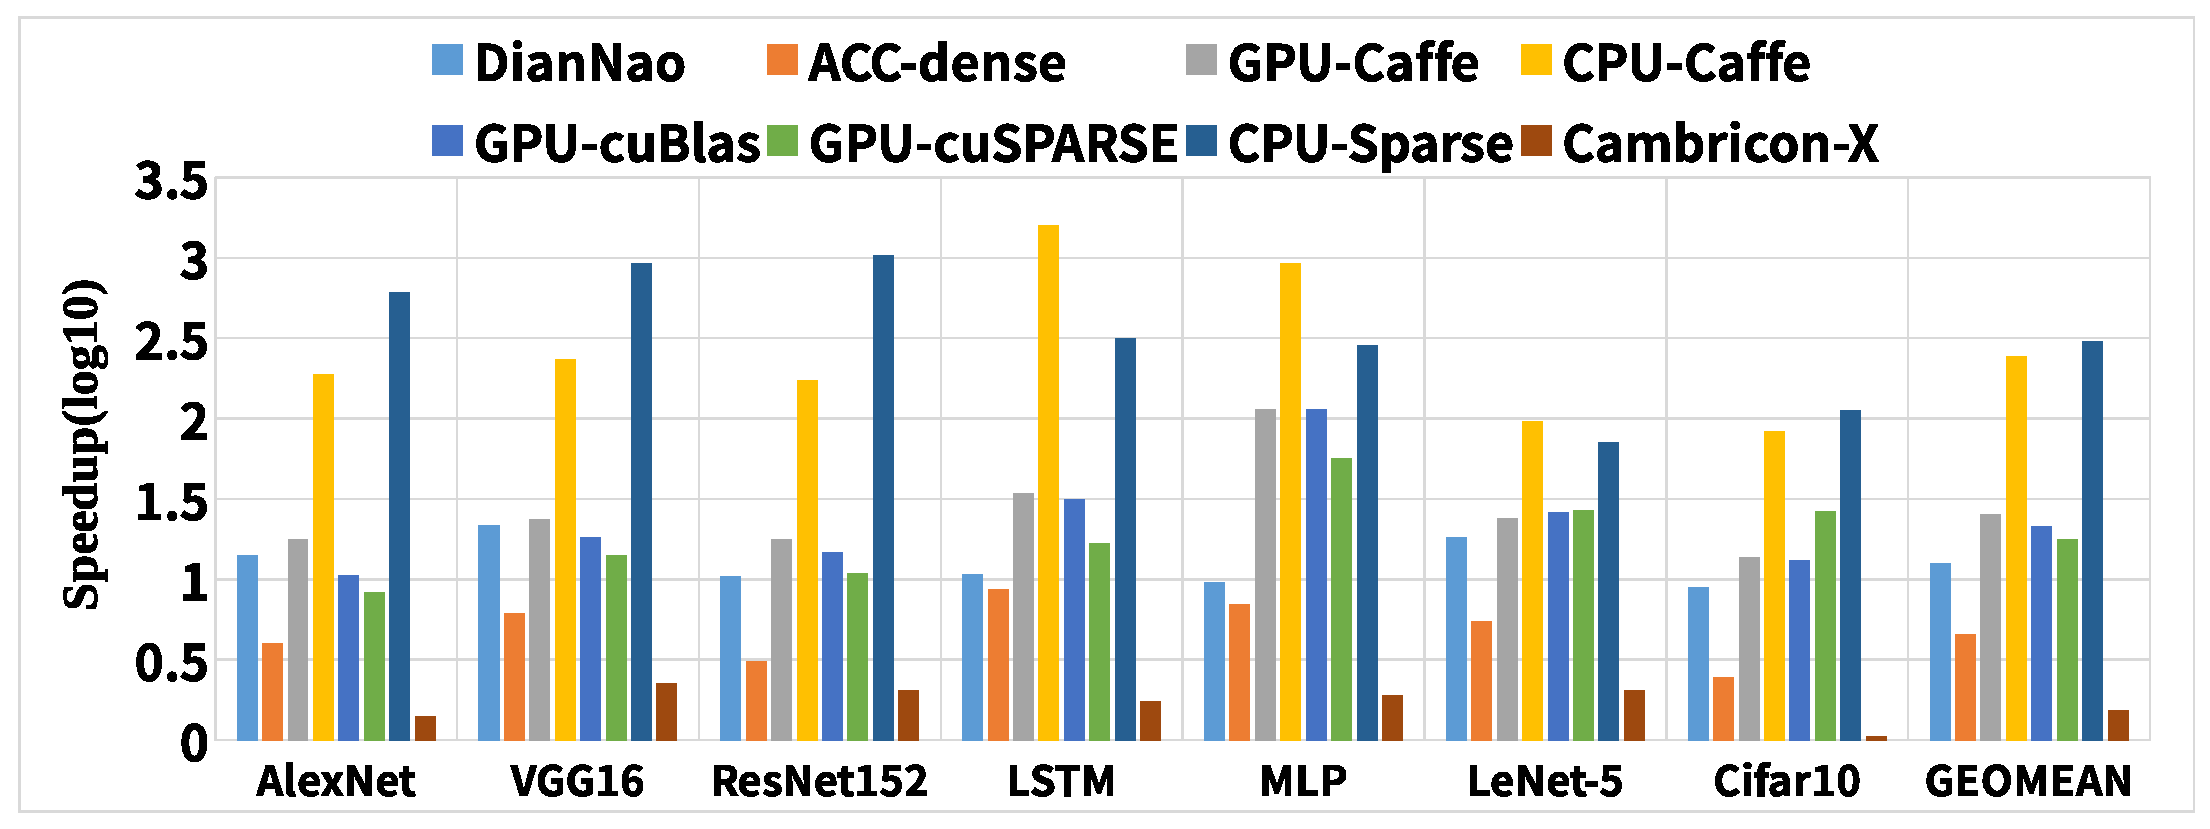
\includegraphics[width=1.0\columnwidth]{total_performance.eps}
\caption{新型加速器与CPU,GPU,DianNao,Cambricon-X的性能对比}
\label{fig:total_performance}
\end{figure}

在图~\ref{fig:total_performance},我们比较了新型加速器,CPU,GPU,DianNao和Cambricon-X的性能,同时,我们将所有性能的数据归一化到了新型加速器在稀疏网络熵的性能。在稠密网络上,新型加速器对比与CPU-Caffe,GPU-Caffe和CPU-cuBLAS分别能够获得44.8倍,5.8倍和5.1倍的加速比。在稀疏网络上,新型加速器对比与CPU-Sparse和GPU-cuSparse分别能够获得331.1倍和19.3倍的加速比。对比于DianNao和Cambricon-X,新型加速器分别能够获得13.10倍和1.71倍加速的加速比。实验结果充分显示了我们的加速器能够充分利用利用神经网络稀疏的特性,从而获得高加速比。值得注意的是,我们的加速器能够通过关闭/开启各个模块(NSM,SSM,WDM,Encoder等),使得加速器能够处理稠密神经网络,稀疏神经网络(包括只利用权值稀疏,只利用神经元稀疏和同时利用神经元/权值稀疏三种情况),局部量化。

新型加速器在处理稀疏神经网络时,对比ACC-dense能够获得4.32倍的加速比,这部分的性能提升主要来自于三个方面。首先,NSM可以充分利用突触稀疏(平均权值稀疏度为$87.99\%$)从而减少计算,最终实现2.06倍的加速比。第二,SSM能够充分利用神经元稀疏(平均神经元稀疏度为$55.41\%$),从而减少神经网络所需的计算量,最终获得1.44倍的加速比。第三,粗粒度稀疏($78.99\%$)和局部量化(减少2.76倍突触数据)可以大大减少片外权值访问量,从而获得1.46倍的加速比

\begin{figure}[h]
\centering
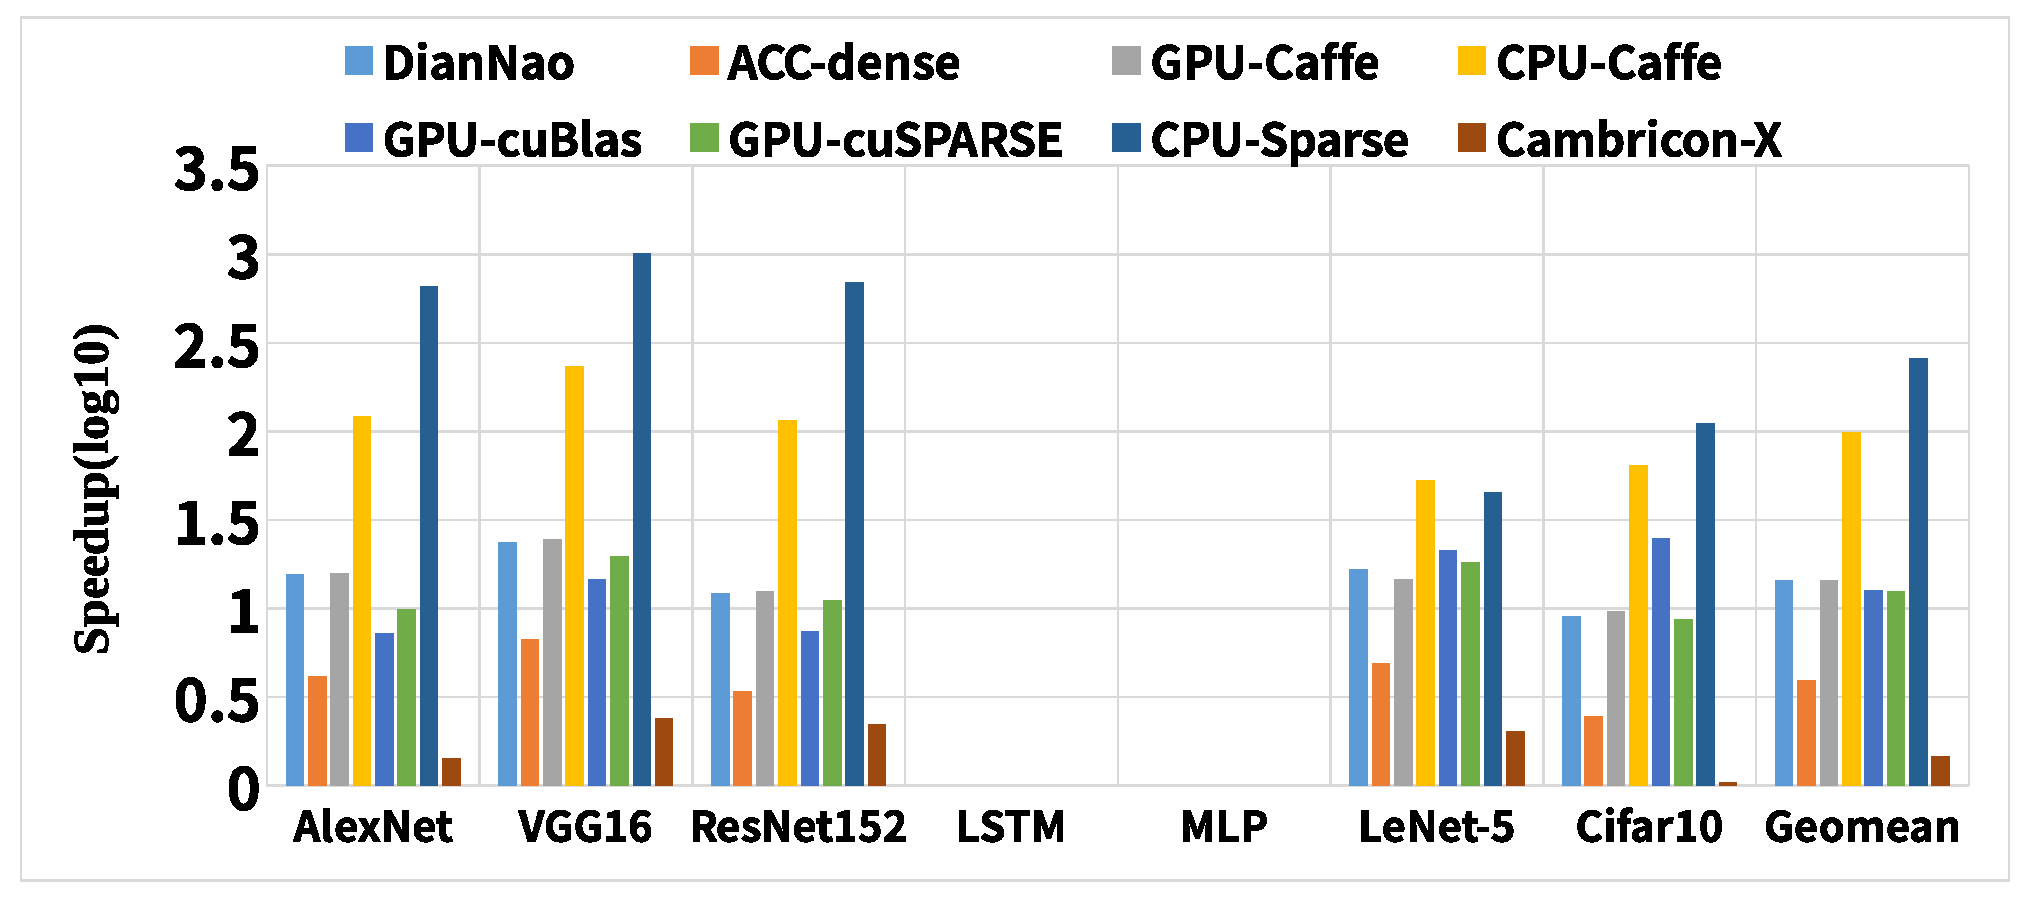
\includegraphics[width=1.0\columnwidth]{conv_performance.eps}
\caption{新型加速器与CPU,GPU,DianNao,Cambricon-X在卷积层上的性能对比}
\label{fig:conv_performance}
\end{figure}

\begin{figure}[h]
\centering
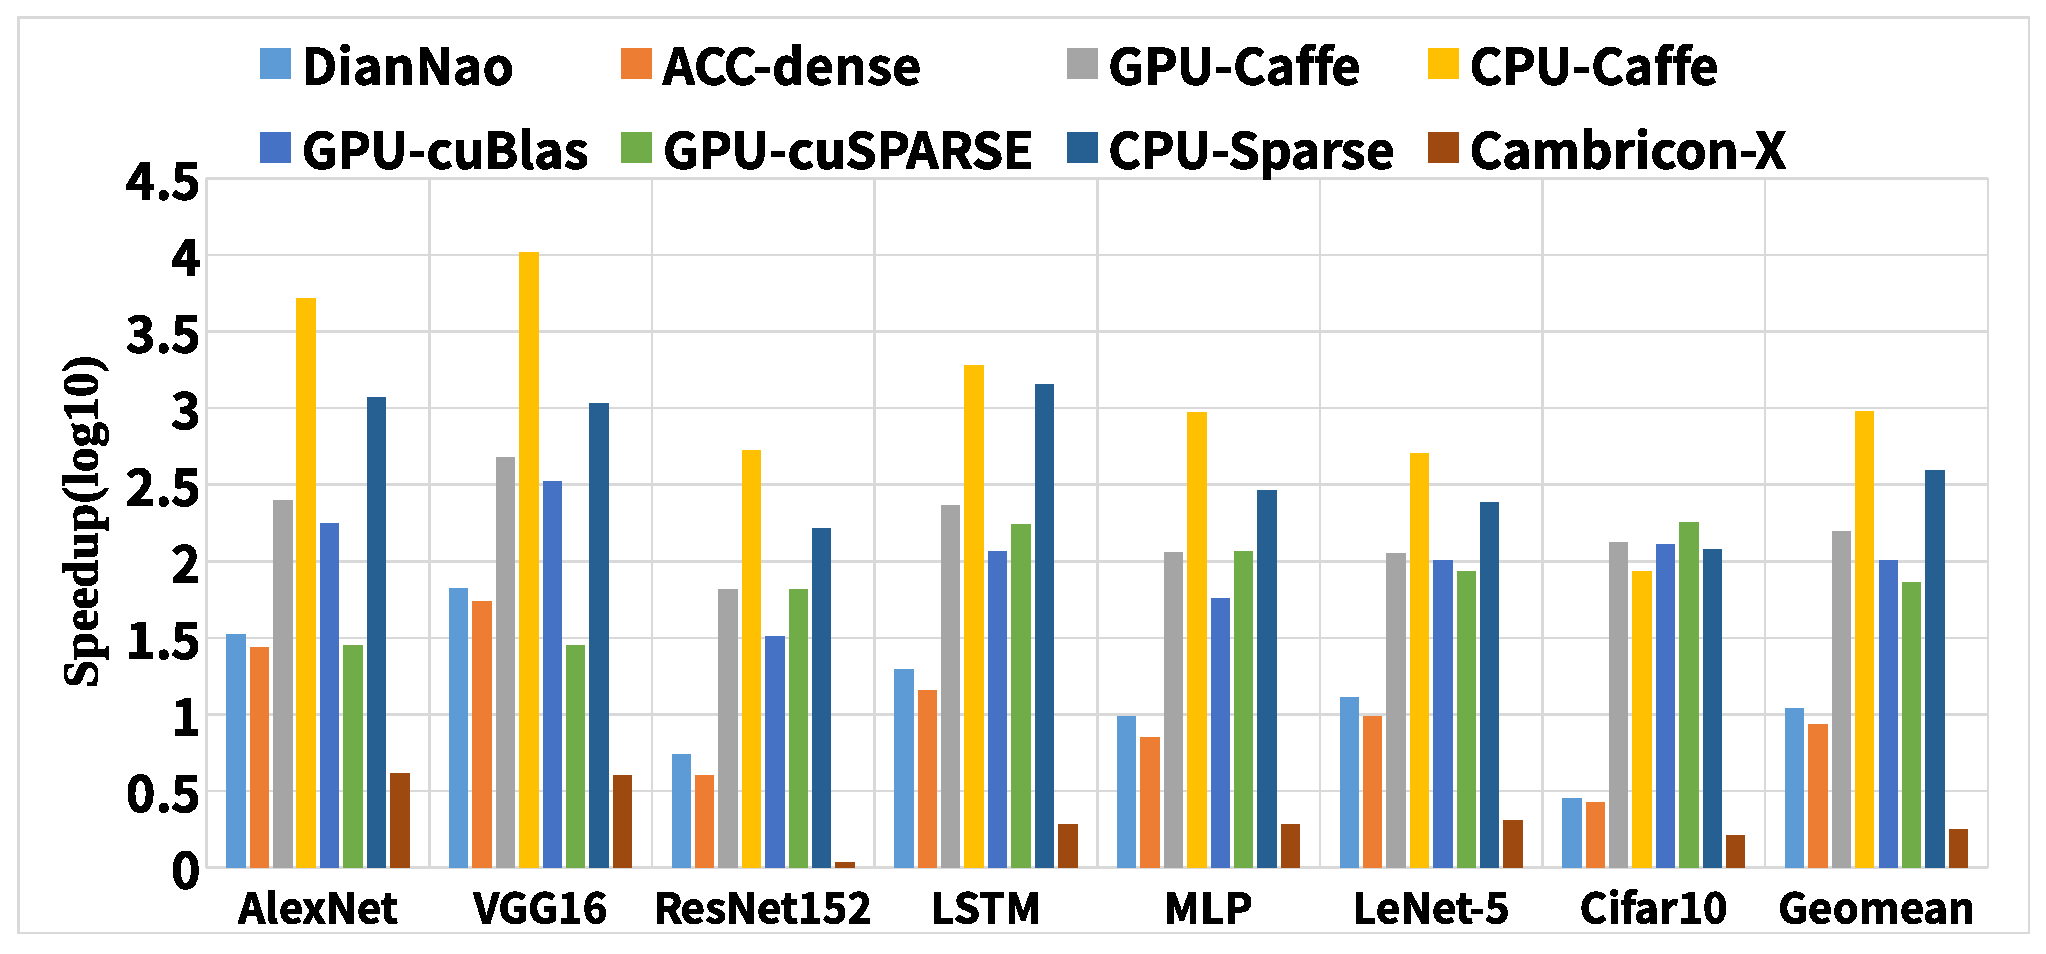
\includegraphics[width=1.0\columnwidth]{fc_performance.eps}
\caption{新型加速器与CPU,GPU,DianNao,Cambricon-X在全连接层上的性能对比}
\label{fig:fc_performance}
\end{figure}

为了进一步探索新型加速器的性能,我们统计了新型加速器在卷积层和全连接层上的性能数据。在卷积层上,对比于CPU-Sparse, GPU-cuSparse和DianNao,我们的加速器分别获得了283.31倍,12.20倍和13.94倍的性能提升;在全连接层上,对比于CPU-Sparse, GPU-cuSparse和DianNao,我们的加速器分别获得了531.89倍,79.05倍和13.56倍的性能提升。值得注意的是,对比于Cambricon-X,我们的加速器能够在卷积层和全连接层分别获得1.66倍和2.15倍的加速比。其中在卷积层上的加速比主要来源于SSM模块能够进一步挖掘神经元稀疏,因为卷积层是计算密集型的层,动态神经元稀疏可以大量减少神经网络中的计算量,例如在AlexNet网络的\emph{conv3}层,稠密情况下需要$52M$的MAC操作(Multiply–accumulate operation),而如果利用$45\%$的动态神经元稀疏,仅仅需要$29M$的MAC操作。在全连接层的性能提升主要来源于权值存储量的减少(局部量化)和索引存储量的减少(索引共享)。WDM能够支持用户自定义比特长度的量化,从而减少突触的存储容量,获得1.77倍的加速比;粗粒度剪枝使得非零位置的索引信息能够被相邻多个输出神经元共享,因此能够额外获得1.21倍的加速比。


\subsection{能耗}
\begin{figure}[h]
\centering
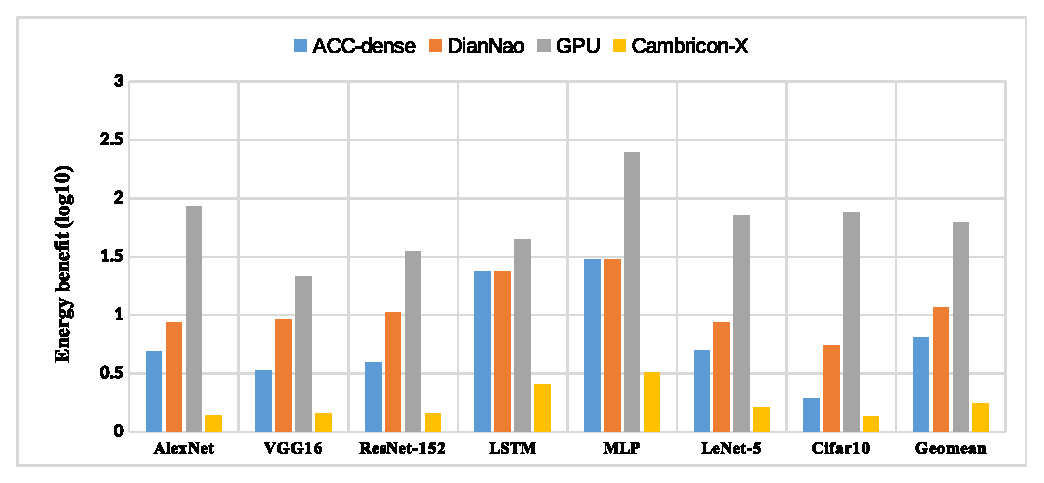
\includegraphics[width=1.0\columnwidth]{energy.eps}
\caption{新型加速器与GPU,DianNao,Cambricon-X在能耗的对比}
\label{fig:energy}
\end{figure}

在七个benchmark上,我们比较了新型加速器,GPU,DianNao和Cambricon-X的能耗,其中我们包括了片外访存的能耗。如图~\ref{fig:energy}所示,对比于GPU,DianNao和Cambricon-X,新型加速器能够减少倍63.49倍,11.72倍和1.75倍的能耗。此外,我们我们观察到局部量化能够减少1.24倍的能耗,动态压缩神经元能够减少1.28倍的能耗。如果不考虑片外访存的能耗,我们加速比分别比GPU,DianNao和Cambricon-X减少1169.51倍,12.30倍和1.75倍能耗。以上实验数据证明我们的加速器能够使用很低的能耗完成神经网络的运算。


\begin{figure}[h]
\centering
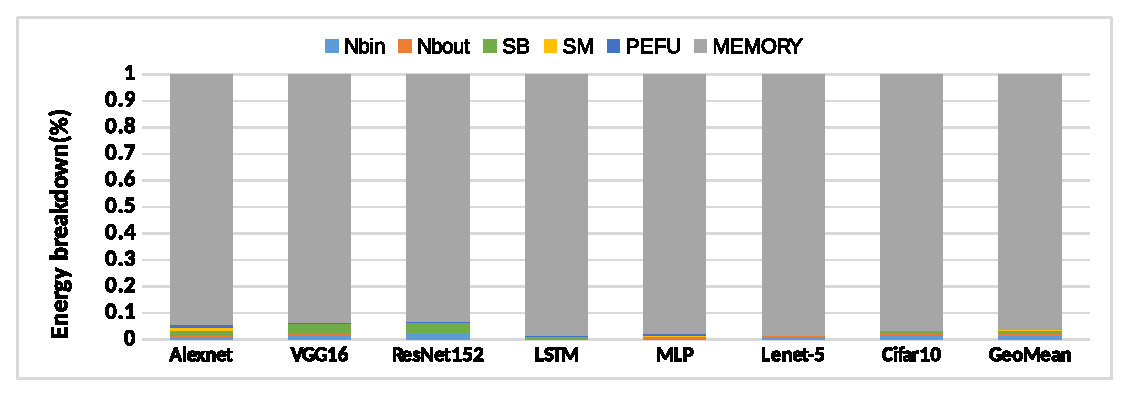
\includegraphics[width=1.0\columnwidth]{energy_breakdown.eps}
\caption{加速器在benchmark上的能耗分布(包括片外访存能耗)}
\label{fig:energy_breakdown}
\end{figure}

我们分析了加速器在七个benchmark上的能耗分布。如图~\ref{fig:energy_breakdown}所示,我们可以观察到片外访存消耗了超过$90\%$的总能量。在LSTM和MLP网络中,这个比例高达$98\%$,远高于其他神经网络,因此这两个网络是访存密集型的网络。实验结果显示,通过稀疏和量化可以显著减少片外访存的能耗。对比于稠密网络,稀疏网络能够减少$72.6\%$的片外访存能耗。

\begin{figure}[h]
\centering
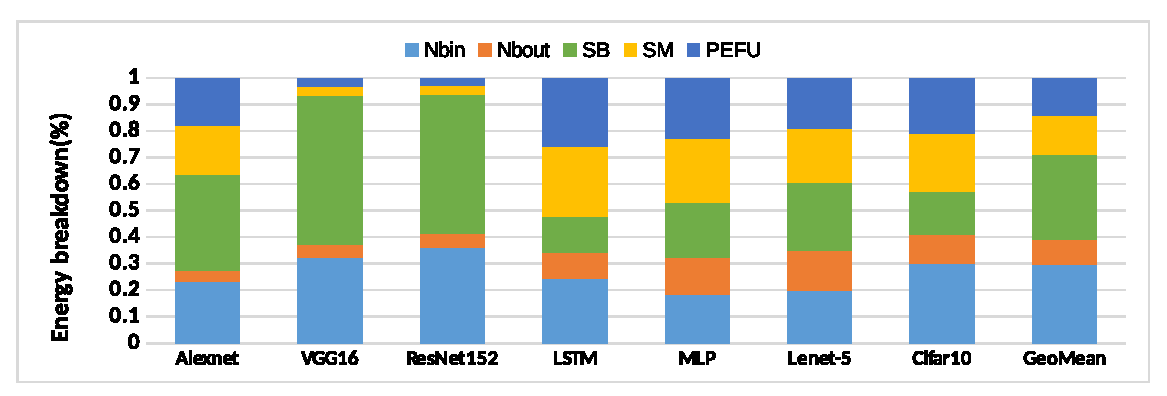
\includegraphics[width=1.0\columnwidth]{energy_breakdown2.eps}
\caption{加速器在benchmark上的能耗分布(不包括片外访存能耗)}
\label{fig:energy_breakdown2}
\end{figure}

我们进一步分析了在不包括片外访存能耗情况下加速器的能耗分布。如图~\ref{fig:energy_breakdown2}所示,片上缓存访问能耗(包括NBin,NBout和SB)平均消耗约$70\%$的总能量,这表明片上缓存访问能耗依然主导片上的能耗。对于LSTM和MLP这两个网络上,片上缓存能耗少于$60\%$,因为在这两个网络中权值不进行重用。对于深层的卷积网络,比如VGG16和ResNet152,片上内存访问能源的比例超过$90\%$,因为在这两个网络中需要复杂的loop tiling和数据重用策略将大规模运算映射到加速器熵。值得注意的是,与Cambricon—X相比,局部量化能够减少2.76倍的权值存储量,从而使得SB减少2.48倍的能耗。

\subsection{讨论}

\subsubsection{熵编码和熵解码模块}
\label{subsubsec:encoding_hw}

目前新型加速器中并没有加入熵解码模块(entropy decoding module)来使得加速器支持权值熵编码,主要是考虑到熵解码模块需要耗费非常大的面积和能耗,但是仅仅能够获得非常有限的性能提升。一个熵解码模块(entropy decoding module)的面积为$6.781*10^{-3}mm^2$,它能够在一个cycle解码出一个码字。由于熵编码是一种变长编码,因此对应的解码模块必须串行进行解码。即使我们可以将数据划分为许多并行的数据流,然后对为每个数据流提供一个熵解码模块,这种方法将会引入巨大的面积和能耗开销。考虑到每一个SB需要在一个cycle提供$T_m\times 4$个数据,为了避免性能损失,我们必须为一个SB提供$T_m\times 4$个熵解码模块,因此我们在加速其中总共需要集成$T_n\times T_m\times 4$个熵解码模块。在$T_m = T_n = 16$的配置下,我们总共需要1024个熵解码模块,这将引入额外$6.94mm^2$的面积和$971.37mW$的功耗,因此加速器的总面积和功耗分别是$13.67mm^2$和$1769.92mW$,分别是原始设计的2.03倍和2.22倍。然而,新增熵解码的加速器在卷积层上几乎没有性能提升,在全连接层也只有1.18倍的性能提升,对比与额外的面积和功耗开销,这种性能提升是非常有限的。因此,我们在加速器中不加入熵解码模块。

\subsubsection{稀疏度与性能}
\begin{figure}[h]
\centering
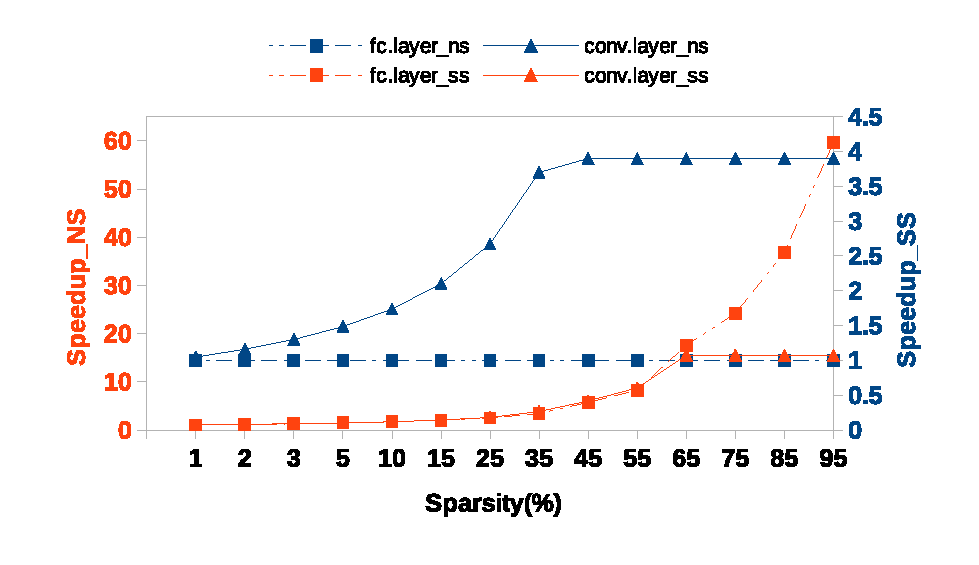
\includegraphics[width=1.0\columnwidth]{sensitivity.eps}
\caption{神经网络稀疏度对加速器性能的影响}
\label{fig:sensitivity}
\end{figure}

我们研究了加速器对神经网络稀疏度的敏感性,即稀疏度对神经网络性能的影响。如图~\ref{fig:sensitivity}所示,我们分别探究了神经元稀疏度和粗粒度权值稀疏度对加速器性能的影响,更进一步的,我们从卷积层和全连接层两个角度进行探究。从图中的数据我们观察到了几个有趣的实验结果:

1)考虑粗粒度权值稀疏,加速器能够在卷积层获得接近理想值的加速比(15.5倍 vs. 16倍)。为了兼容大多数网络的权值稀疏度~\ref{tab:sparsities},我们将NSM设计成为256选16的结构,即NSM最多从256个输入神经元中筛选出16个需要进行计算的神经元,从而最多实现16倍的加速器。我们的加速器能够接近理想加速器的主要原因是我们使用pingpong的模式管理片上缓存,使得加速器的片外访存延迟能够被运算时间覆盖。值得注意的是,由于我们的加速器能够充分利用粗粒度稀疏实现负载均衡,因此在相同稀疏度情况下,新型加速器能够获得比Cambricon-X更优的加速比。

2)考虑粗粒度权值稀疏,在全连接层中,新型加速器能够很容易地在低稀疏度情况下(低于$5\%$)获得加速比,并且随着稀疏度的提高,加速比也会不断提高,在稀疏度为$99\%$时能够获得59.59倍的加速比。主要原因是全连接层是一个访存密集的层,压缩后的权值能够大大减少片外访存数据量,从而减少片外访存时间,减少总执行时间。

3)考虑神经元稀疏,新型加速器在卷积层最高能够获得3.9倍的加速比,接近理想的4倍加速比。由于在大多数情况下,神经元的稠密度高于$25\%$(稀疏度低于$75\%$),我们将SSM设计成为64选16的结构,因此最多获得4倍的加速比。这个设计能够满足绝大多数神经网络的需求。

4)神经元稀疏并不能在全连接层带来性能的提升,因此在全连接层片外权值访存时间主导了总执行时间(超过$99\%$),而神经元稀疏并不能有效地减少内存访问。

上述的实验结果进一步验证了新型加速器能够高效地利用神经网络中神经元稀疏和权值稀疏。

\subsubsection{减少的不规则度}
减少稀疏神经元的不规则度能够对加速器的设计,性能产生深远的影响。第一,减少不规则度能够简化加速器的设计。我们可以使用一个共享的NSM取代$T_n$个分布式的NSM,从而节省$10.35mm^2$的面积和$1821.9mW$的功耗;同时我们可以用一个共享的SIB来代替16个独立的SIB,从而节省$15KB$的SRAM大小。第二,减少不规则度能够大大减少权值索引的规模(26.83倍),从而获得1.06倍的加速比,减少1.11倍的能耗。

\subsubsection{类似粗粒度稀疏的方法}
最近有不少类似于粗粒度稀疏的研究,例如SIMD-aware weight pruning~\cite{yu2017scalpel},synapse vector elimination~\cite{hill2017deftnn},channel reduction和filter reduction~\cite{wen2016learning,lebedev2016fast}。尽管这些技术可以减少稀疏神经网络的不规则度,从而简化加速器设计,但是通常会导致显著的精度损失~\cite{li2016pruning}。

\citet{mao2017exploring}探究了一些列结构化稀疏的方法,包括细粒度稀疏(fine-grained sparsity),向量层次稀疏(vector-level sparsity),卷积核层次稀疏(kernel-level sparsity)和过滤器层次稀疏(filter-level sparsity),同时评估这些稀疏方法对神经网络不规则度和精度的影响。 值得注意的是,我们提出的粗粒度剪枝方式并不会限制剪枝块的规模,因此是一种普遍性的剪枝方法。通过指定参数,粗粒度剪枝能够达到上述各种形式稀疏的效果。

\subsubsection{其他稀疏神经网络加速器}
EIE~\cite{han2016eie}能够加速稀疏神经网络的全连接层,它采用CSC的压缩方式压缩权值。为了能够完全消除片外访存,它使用非常大的片上缓存存储所有的突触。为了使AlexNet网络的全连接层权值能够完全存储在片上缓存,EIE的总面积需要达到$40.8mm^2$,是我们加速器的面积的5.07倍。同时,EIE只支持固定比特的量化,而新型加速器中的WDM能够支持自定义比特的量化,从而权衡神经网络的压缩效果和精度。为了公平地与EIE比较性能,我们假设加速器的片上缓存足够大,能够存储全连接层的所有权值,因此我们将加速器的性能聚焦在计算时间。如表~\ref{tab:EIE}所示,相比于EIE,新型加速器能够平均获得1.65倍的加速比。

\begin{table}[h]
\centering
\caption{\footnotesize 与EIE的性能比较 \emph{(microsecond)}.}
\label{tab:EIE}
\begin{tabular}{@{}lll@{~~}lll@{~~}lll@{~~}lll@{~~}lll@{~~}lll@{~~}lll@{~~}lllllll}
\toprule
layer & \multicolumn{3}{c}{AlexNet} & \multicolumn{3}{c}{VGG16} & Geomean\\
& fc6 & fc7 & fc8 & fc6 & fc7 & fc8     \\
\midrule
EIE & 30.30 & 12.20 & 9.90  & 34.40 & 8.70  & 7.50  & --\\
ACC & 18.43 & 8.19  & 5.13  & 25.23 & 4.12  & 5.09  & --\\
Speedup & $1.64\times$ & $1.49\times$ & $1.93\times$ & $1.36\times$ & $2.11\times$ & $1.49\times$ & $1.65\times$ \\
\bottomrule
\end{tabular}
\end{table}

新型加速器与Cambricon-X~\cite{zhang2016cambricon}都是用了索引的方式利用神经网络的稀疏性质,但是新型加速器索引方式与Cambricon-X有三个方面不同。首先,新型加速器包含一个共享的索引模块(NSM),它能够充分挖掘权值的粗粒度稀疏特性。由于粗粒度稀疏,加速器的各个PE共享相同的索引,因此NSM筛选出的神经元能够被PE共享,从而减少索引模块开销以及NSM与PE之间的带宽需求。第二,新型加速器的PE中集成了一个本地的权值索引模块(SSM),从而充分利用神经元稀疏。虽然粗粒度稀疏能够减少稀疏神经网络的不规则性,但是稀疏的神经元依然存在不规则性,例如ReLU激励能够使得许多神经元的激励为“0”,SSM模块能够最小化这种不规则性的影响。因此新型索引模块能够充分利用神经元稀疏和权值稀疏,而Cambricon-X只能利用权值稀疏。第三,新型加速器中集成了Encoder模块,动态压缩稀疏的神经元,从而减少片外神经元访问。实验显示,Encoder模块能够进一步减少1.28倍的能耗;更具体地说,它能够在卷积层和全连接层分别减少1.68倍和1.02倍的能耗。第四,加速器的每一个PE中集成了WDM模块用于解码量化后的权值,从而充分利用局部量化,进一步减少片外权值访问量。

SCNN~\cite{angshuman2017scnn}能够挖掘权值稀疏和神经元稀疏,对比于稠密神经网络,它能够获得2.7倍的加速比,同时减少2.3倍的能耗。而我们加速器能够获得4.32倍的加速比,减少6.53倍的能耗,这充分显示了我们加速器高性能和低能耗的特点。

